\documentclass[11pt]{article}
\usepackage{ACL}
\usepackage{times}
\usepackage{url}
\usepackage{latexsym}
\usepackage{enumitem}
\usepackage{subfigure}
\usepackage{graphicx}
%%%%% NEW MATH DEFINITIONS %%%%%

\usepackage{amsmath,amsfonts,bm}

% Mark sections of captions for referring to divisions of figures
\newcommand{\figleft}{{\em (Left)}}
\newcommand{\figcenter}{{\em (Center)}}
\newcommand{\figright}{{\em (Right)}}
\newcommand{\figtop}{{\em (Top)}}
\newcommand{\figbottom}{{\em (Bottom)}}
\newcommand{\captiona}{{\em (a)}}
\newcommand{\captionb}{{\em (b)}}
\newcommand{\captionc}{{\em (c)}}
\newcommand{\captiond}{{\em (d)}}

% Highlight a newly defined term
\newcommand{\newterm}[1]{{\bf #1}}


% Figure reference, lower-case.
\def\figref#1{figure~\ref{#1}}
% Figure reference, capital. For start of sentence
\def\Figref#1{Figure~\ref{#1}}
\def\twofigref#1#2{figures \ref{#1} and \ref{#2}}
\def\quadfigref#1#2#3#4{figures \ref{#1}, \ref{#2}, \ref{#3} and \ref{#4}}
% Section reference, lower-case.
\def\secref#1{section~\ref{#1}}
% Section reference, capital.
\def\Secref#1{Section~\ref{#1}}
% Reference to two sections.
\def\twosecrefs#1#2{sections \ref{#1} and \ref{#2}}
% Reference to three sections.
\def\secrefs#1#2#3{sections \ref{#1}, \ref{#2} and \ref{#3}}
% Reference to an equation, lower-case.
\def\eqref#1{equation~\ref{#1}}
% Reference to an equation, upper case
\def\Eqref#1{Equation~\ref{#1}}
% A raw reference to an equation---avoid using if possible
\def\plaineqref#1{\ref{#1}}
% Reference to a chapter, lower-case.
\def\chapref#1{chapter~\ref{#1}}
% Reference to an equation, upper case.
\def\Chapref#1{Chapter~\ref{#1}}
% Reference to a range of chapters
\def\rangechapref#1#2{chapters\ref{#1}--\ref{#2}}
% Reference to an algorithm, lower-case.
\def\algref#1{algorithm~\ref{#1}}
% Reference to an algorithm, upper case.
\def\Algref#1{Algorithm~\ref{#1}}
\def\twoalgref#1#2{algorithms \ref{#1} and \ref{#2}}
\def\Twoalgref#1#2{Algorithms \ref{#1} and \ref{#2}}
% Reference to a part, lower case
\def\partref#1{part~\ref{#1}}
% Reference to a part, upper case
\def\Partref#1{Part~\ref{#1}}
\def\twopartref#1#2{parts \ref{#1} and \ref{#2}}

\def\ceil#1{\lceil #1 \rceil}
\def\floor#1{\lfloor #1 \rfloor}
\def\1{\bm{1}}
\newcommand{\train}{\mathcal{D}}
\newcommand{\valid}{\mathcal{D_{\mathrm{valid}}}}
\newcommand{\test}{\mathcal{D_{\mathrm{test}}}}

\def\eps{{\epsilon}}


% Random variables
\def\reta{{\textnormal{$\eta$}}}
\def\ra{{\textnormal{a}}}
\def\rb{{\textnormal{b}}}
\def\rc{{\textnormal{c}}}
\def\rd{{\textnormal{d}}}
\def\re{{\textnormal{e}}}
\def\rf{{\textnormal{f}}}
\def\rg{{\textnormal{g}}}
\def\rh{{\textnormal{h}}}
\def\ri{{\textnormal{i}}}
\def\rj{{\textnormal{j}}}
\def\rk{{\textnormal{k}}}
\def\rl{{\textnormal{l}}}
% rm is already a command, just don't name any random variables m
\def\rn{{\textnormal{n}}}
\def\ro{{\textnormal{o}}}
\def\rp{{\textnormal{p}}}
\def\rq{{\textnormal{q}}}
\def\rr{{\textnormal{r}}}
\def\rs{{\textnormal{s}}}
\def\rt{{\textnormal{t}}}
\def\ru{{\textnormal{u}}}
\def\rv{{\textnormal{v}}}
\def\rw{{\textnormal{w}}}
\def\rx{{\textnormal{x}}}
\def\ry{{\textnormal{y}}}
\def\rz{{\textnormal{z}}}

% Random vectors
\def\rvepsilon{{\mathbf{\epsilon}}}
\def\rvtheta{{\mathbf{\theta}}}
\def\rva{{\mathbf{a}}}
\def\rvb{{\mathbf{b}}}
\def\rvc{{\mathbf{c}}}
\def\rvd{{\mathbf{d}}}
\def\rve{{\mathbf{e}}}
\def\rvf{{\mathbf{f}}}
\def\rvg{{\mathbf{g}}}
\def\rvh{{\mathbf{h}}}
\def\rvu{{\mathbf{i}}}
\def\rvj{{\mathbf{j}}}
\def\rvk{{\mathbf{k}}}
\def\rvl{{\mathbf{l}}}
\def\rvm{{\mathbf{m}}}
\def\rvn{{\mathbf{n}}}
\def\rvo{{\mathbf{o}}}
\def\rvp{{\mathbf{p}}}
\def\rvq{{\mathbf{q}}}
\def\rvr{{\mathbf{r}}}
\def\rvs{{\mathbf{s}}}
\def\rvt{{\mathbf{t}}}
\def\rvu{{\mathbf{u}}}
\def\rvv{{\mathbf{v}}}
\def\rvw{{\mathbf{w}}}
\def\rvx{{\mathbf{x}}}
\def\rvy{{\mathbf{y}}}
\def\rvz{{\mathbf{z}}}

% Elements of random vectors
\def\erva{{\textnormal{a}}}
\def\ervb{{\textnormal{b}}}
\def\ervc{{\textnormal{c}}}
\def\ervd{{\textnormal{d}}}
\def\erve{{\textnormal{e}}}
\def\ervf{{\textnormal{f}}}
\def\ervg{{\textnormal{g}}}
\def\ervh{{\textnormal{h}}}
\def\ervi{{\textnormal{i}}}
\def\ervj{{\textnormal{j}}}
\def\ervk{{\textnormal{k}}}
\def\ervl{{\textnormal{l}}}
\def\ervm{{\textnormal{m}}}
\def\ervn{{\textnormal{n}}}
\def\ervo{{\textnormal{o}}}
\def\ervp{{\textnormal{p}}}
\def\ervq{{\textnormal{q}}}
\def\ervr{{\textnormal{r}}}
\def\ervs{{\textnormal{s}}}
\def\ervt{{\textnormal{t}}}
\def\ervu{{\textnormal{u}}}
\def\ervv{{\textnormal{v}}}
\def\ervw{{\textnormal{w}}}
\def\ervx{{\textnormal{x}}}
\def\ervy{{\textnormal{y}}}
\def\ervz{{\textnormal{z}}}

% Random matrices
\def\rmA{{\mathbf{A}}}
\def\rmB{{\mathbf{B}}}
\def\rmC{{\mathbf{C}}}
\def\rmD{{\mathbf{D}}}
\def\rmE{{\mathbf{E}}}
\def\rmF{{\mathbf{F}}}
\def\rmG{{\mathbf{G}}}
\def\rmH{{\mathbf{H}}}
\def\rmI{{\mathbf{I}}}
\def\rmJ{{\mathbf{J}}}
\def\rmK{{\mathbf{K}}}
\def\rmL{{\mathbf{L}}}
\def\rmM{{\mathbf{M}}}
\def\rmN{{\mathbf{N}}}
\def\rmO{{\mathbf{O}}}
\def\rmP{{\mathbf{P}}}
\def\rmQ{{\mathbf{Q}}}
\def\rmR{{\mathbf{R}}}
\def\rmS{{\mathbf{S}}}
\def\rmT{{\mathbf{T}}}
\def\rmU{{\mathbf{U}}}
\def\rmV{{\mathbf{V}}}
\def\rmW{{\mathbf{W}}}
\def\rmX{{\mathbf{X}}}
\def\rmY{{\mathbf{Y}}}
\def\rmZ{{\mathbf{Z}}}

% Elements of random matrices
\def\ermA{{\textnormal{A}}}
\def\ermB{{\textnormal{B}}}
\def\ermC{{\textnormal{C}}}
\def\ermD{{\textnormal{D}}}
\def\ermE{{\textnormal{E}}}
\def\ermF{{\textnormal{F}}}
\def\ermG{{\textnormal{G}}}
\def\ermH{{\textnormal{H}}}
\def\ermI{{\textnormal{I}}}
\def\ermJ{{\textnormal{J}}}
\def\ermK{{\textnormal{K}}}
\def\ermL{{\textnormal{L}}}
\def\ermM{{\textnormal{M}}}
\def\ermN{{\textnormal{N}}}
\def\ermO{{\textnormal{O}}}
\def\ermP{{\textnormal{P}}}
\def\ermQ{{\textnormal{Q}}}
\def\ermR{{\textnormal{R}}}
\def\ermS{{\textnormal{S}}}
\def\ermT{{\textnormal{T}}}
\def\ermU{{\textnormal{U}}}
\def\ermV{{\textnormal{V}}}
\def\ermW{{\textnormal{W}}}
\def\ermX{{\textnormal{X}}}
\def\ermY{{\textnormal{Y}}}
\def\ermZ{{\textnormal{Z}}}

% Vectors
\def\vzero{{\bm{0}}}
\def\vone{{\bm{1}}}
\def\vmu{{\bm{\mu}}}
\def\vtheta{{\bm{\theta}}}
\def\va{{\bm{a}}}
\def\vb{{\bm{b}}}
\def\vc{{\bm{c}}}
\def\vd{{\bm{d}}}
\def\ve{{\bm{e}}}
\def\vf{{\bm{f}}}
\def\vg{{\bm{g}}}
\def\vh{{\bm{h}}}
\def\vi{{\bm{i}}}
\def\vj{{\bm{j}}}
\def\vk{{\bm{k}}}
\def\vl{{\bm{l}}}
\def\vm{{\bm{m}}}
\def\vn{{\bm{n}}}
\def\vo{{\bm{o}}}
\def\vp{{\bm{p}}}
\def\vq{{\bm{q}}}
\def\vr{{\bm{r}}}
\def\vs{{\bm{s}}}
\def\vt{{\bm{t}}}
\def\vu{{\bm{u}}}
\def\vv{{\bm{v}}}
\def\vw{{\bm{w}}}
\def\vx{{\bm{x}}}
\def\vy{{\bm{y}}}
\def\vz{{\bm{z}}}

% Elements of vectors
\def\evalpha{{\alpha}}
\def\evbeta{{\beta}}
\def\evepsilon{{\epsilon}}
\def\evlambda{{\lambda}}
\def\evomega{{\omega}}
\def\evmu{{\mu}}
\def\evpsi{{\psi}}
\def\evsigma{{\sigma}}
\def\evtheta{{\theta}}
\def\eva{{a}}
\def\evb{{b}}
\def\evc{{c}}
\def\evd{{d}}
\def\eve{{e}}
\def\evf{{f}}
\def\evg{{g}}
\def\evh{{h}}
\def\evi{{i}}
\def\evj{{j}}
\def\evk{{k}}
\def\evl{{l}}
\def\evm{{m}}
\def\evn{{n}}
\def\evo{{o}}
\def\evp{{p}}
\def\evq{{q}}
\def\evr{{r}}
\def\evs{{s}}
\def\evt{{t}}
\def\evu{{u}}
\def\evv{{v}}
\def\evw{{w}}
\def\evx{{x}}
\def\evy{{y}}
\def\evz{{z}}

% Matrix
\def\mA{{\bm{A}}}
\def\mB{{\bm{B}}}
\def\mC{{\bm{C}}}
\def\mD{{\bm{D}}}
\def\mE{{\bm{E}}}
\def\mF{{\bm{F}}}
\def\mG{{\bm{G}}}
\def\mH{{\bm{H}}}
\def\mI{{\bm{I}}}
\def\mJ{{\bm{J}}}
\def\mK{{\bm{K}}}
\def\mL{{\bm{L}}}
\def\mM{{\bm{M}}}
\def\mN{{\bm{N}}}
\def\mO{{\bm{O}}}
\def\mP{{\bm{P}}}
\def\mQ{{\bm{Q}}}
\def\mR{{\bm{R}}}
\def\mS{{\bm{S}}}
\def\mT{{\bm{T}}}
\def\mU{{\bm{U}}}
\def\mV{{\bm{V}}}
\def\mW{{\bm{W}}}
\def\mX{{\bm{X}}}
\def\mY{{\bm{Y}}}
\def\mZ{{\bm{Z}}}
\def\mBeta{{\bm{\beta}}}
\def\mPhi{{\bm{\Phi}}}
\def\mLambda{{\bm{\Lambda}}}
\def\mSigma{{\bm{\Sigma}}}

% Tensor
\DeclareMathAlphabet{\mathsfit}{\encodingdefault}{\sfdefault}{m}{sl}
\SetMathAlphabet{\mathsfit}{bold}{\encodingdefault}{\sfdefault}{bx}{n}
\newcommand{\tens}[1]{\bm{\mathsfit{#1}}}
\def\tA{{\tens{A}}}
\def\tB{{\tens{B}}}
\def\tC{{\tens{C}}}
\def\tD{{\tens{D}}}
\def\tE{{\tens{E}}}
\def\tF{{\tens{F}}}
\def\tG{{\tens{G}}}
\def\tH{{\tens{H}}}
\def\tI{{\tens{I}}}
\def\tJ{{\tens{J}}}
\def\tK{{\tens{K}}}
\def\tL{{\tens{L}}}
\def\tM{{\tens{M}}}
\def\tN{{\tens{N}}}
\def\tO{{\tens{O}}}
\def\tP{{\tens{P}}}
\def\tQ{{\tens{Q}}}
\def\tR{{\tens{R}}}
\def\tS{{\tens{S}}}
\def\tT{{\tens{T}}}
\def\tU{{\tens{U}}}
\def\tV{{\tens{V}}}
\def\tW{{\tens{W}}}
\def\tX{{\tens{X}}}
\def\tY{{\tens{Y}}}
\def\tZ{{\tens{Z}}}


% Graph
\def\gA{{\mathcal{A}}}
\def\gB{{\mathcal{B}}}
\def\gC{{\mathcal{C}}}
\def\gD{{\mathcal{D}}}
\def\gE{{\mathcal{E}}}
\def\gF{{\mathcal{F}}}
\def\gG{{\mathcal{G}}}
\def\gH{{\mathcal{H}}}
\def\gI{{\mathcal{I}}}
\def\gJ{{\mathcal{J}}}
\def\gK{{\mathcal{K}}}
\def\gL{{\mathcal{L}}}
\def\gM{{\mathcal{M}}}
\def\gN{{\mathcal{N}}}
\def\gO{{\mathcal{O}}}
\def\gP{{\mathcal{P}}}
\def\gQ{{\mathcal{Q}}}
\def\gR{{\mathcal{R}}}
\def\gS{{\mathcal{S}}}
\def\gT{{\mathcal{T}}}
\def\gU{{\mathcal{U}}}
\def\gV{{\mathcal{V}}}
\def\gW{{\mathcal{W}}}
\def\gX{{\mathcal{X}}}
\def\gY{{\mathcal{Y}}}
\def\gZ{{\mathcal{Z}}}

% Sets
\def\sA{{\mathbb{A}}}
\def\sB{{\mathbb{B}}}
\def\sC{{\mathbb{C}}}
\def\sD{{\mathbb{D}}}
% Don't use a set called E, because this would be the same as our symbol
% for expectation.
\def\sF{{\mathbb{F}}}
\def\sG{{\mathbb{G}}}
\def\sH{{\mathbb{H}}}
\def\sI{{\mathbb{I}}}
\def\sJ{{\mathbb{J}}}
\def\sK{{\mathbb{K}}}
\def\sL{{\mathbb{L}}}
\def\sM{{\mathbb{M}}}
\def\sN{{\mathbb{N}}}
\def\sO{{\mathbb{O}}}
\def\sP{{\mathbb{P}}}
\def\sQ{{\mathbb{Q}}}
\def\sR{{\mathbb{R}}}
\def\sS{{\mathbb{S}}}
\def\sT{{\mathbb{T}}}
\def\sU{{\mathbb{U}}}
\def\sV{{\mathbb{V}}}
\def\sW{{\mathbb{W}}}
\def\sX{{\mathbb{X}}}
\def\sY{{\mathbb{Y}}}
\def\sZ{{\mathbb{Z}}}

% Entries of a matrix
\def\emLambda{{\Lambda}}
\def\emA{{A}}
\def\emB{{B}}
\def\emC{{C}}
\def\emD{{D}}
\def\emE{{E}}
\def\emF{{F}}
\def\emG{{G}}
\def\emH{{H}}
\def\emI{{I}}
\def\emJ{{J}}
\def\emK{{K}}
\def\emL{{L}}
\def\emM{{M}}
\def\emN{{N}}
\def\emO{{O}}
\def\emP{{P}}
\def\emQ{{Q}}
\def\emR{{R}}
\def\emS{{S}}
\def\emT{{T}}
\def\emU{{U}}
\def\emV{{V}}
\def\emW{{W}}
\def\emX{{X}}
\def\emY{{Y}}
\def\emZ{{Z}}
\def\emSigma{{\Sigma}}

% entries of a tensor
% Same font as tensor, without \bm wrapper
\newcommand{\etens}[1]{\mathsfit{#1}}
\def\etLambda{{\etens{\Lambda}}}
\def\etA{{\etens{A}}}
\def\etB{{\etens{B}}}
\def\etC{{\etens{C}}}
\def\etD{{\etens{D}}}
\def\etE{{\etens{E}}}
\def\etF{{\etens{F}}}
\def\etG{{\etens{G}}}
\def\etH{{\etens{H}}}
\def\etI{{\etens{I}}}
\def\etJ{{\etens{J}}}
\def\etK{{\etens{K}}}
\def\etL{{\etens{L}}}
\def\etM{{\etens{M}}}
\def\etN{{\etens{N}}}
\def\etO{{\etens{O}}}
\def\etP{{\etens{P}}}
\def\etQ{{\etens{Q}}}
\def\etR{{\etens{R}}}
\def\etS{{\etens{S}}}
\def\etT{{\etens{T}}}
\def\etU{{\etens{U}}}
\def\etV{{\etens{V}}}
\def\etW{{\etens{W}}}
\def\etX{{\etens{X}}}
\def\etY{{\etens{Y}}}
\def\etZ{{\etens{Z}}}

% The true underlying data generating distribution
\newcommand{\pdata}{p_{\rm{data}}}
% The empirical distribution defined by the training set
\newcommand{\ptrain}{\hat{p}_{\rm{data}}}
\newcommand{\Ptrain}{\hat{P}_{\rm{data}}}
% The model distribution
\newcommand{\pmodel}{p_{\rm{model}}}
\newcommand{\Pmodel}{P_{\rm{model}}}
\newcommand{\ptildemodel}{\tilde{p}_{\rm{model}}}
% Stochastic autoencoder distributions
\newcommand{\pencode}{p_{\rm{encoder}}}
\newcommand{\pdecode}{p_{\rm{decoder}}}
\newcommand{\precons}{p_{\rm{reconstruct}}}

\newcommand{\laplace}{\mathrm{Laplace}} % Laplace distribution

\DeclareMathOperator{\E}{\mathbb{E}}
\newcommand{\Ls}{\mathcal{L}}
\newcommand{\R}{\mathbb{R}}
\newcommand{\emp}{\tilde{p}}
\newcommand{\lr}{\alpha}
\newcommand{\reg}{\lambda}
\newcommand{\rect}{\mathrm{rectifier}}
\newcommand{\softmax}{\mathrm{softmax}}
\newcommand{\sigmoid}{\sigma}
\newcommand{\softplus}{\zeta}
\newcommand{\KL}{D_{\mathrm{KL}}}
\newcommand{\Var}{\mathrm{Var}}
\newcommand{\standarderror}{\mathrm{SE}}
\newcommand{\Cov}{\mathrm{Cov}}
% Wolfram Mathworld says $L^2$ is for function spaces and $\ell^2$ is for vectors
% But then they seem to use $L^2$ for vectors throughout the site, and so does
% wikipedia.
\newcommand{\normlzero}{L^0}
\newcommand{\normlone}{L^1}
\newcommand{\normltwo}{L^2}
\newcommand{\normlp}{L^p}
\newcommand{\normmax}{L^\infty}

\newcommand{\parents}{Pa} % See usage in notation.tex. Chosen to match Daphne's book.

\DeclareMathOperator*{\argmax}{arg\,max}
\DeclareMathOperator*{\argmin}{arg\,min}

\DeclareMathOperator{\sign}{sign}
\DeclareMathOperator{\Tr}{Tr}
\let\ab\allowbreak

\usepackage{bbm}
\usepackage{amssymb}
\usepackage{amsmath}
\allowdisplaybreaks
\usepackage{cancel}
\usepackage[switch]{lineno}
\usepackage[bottom]{footmisc}
\usepackage[ruled,vlined,linesnumbered]{algorithm2e}

\definecolor{orange}{rgb}{0.93, 0.53, 0.18}

\aclfinalcopy % Uncomment this line for the final submission
%\def\aclpaperid{***} %  Enter the acl Paper ID here


\title{On developmental and communicative constraints on the world's colour systems}

% 2. Two rows of authors (set titlebox length to 7cm)
%
\author{First Author \\
 \\\And
 Second Author \\
 \\\AND
 Third Author \\
 \\\And
 Fourth Author \\
 }

\date{}

\begin{document}
\maketitle
\pagestyle{plain} %remove before sub
\thispagestyle{plain} %remove before sub
\linenumbers %remove before sub
\begin{abstract}
The attested colour systems in the world's languages show many remarkable similarities. 
Previous studies have attempted to explain this in terms how efficient the systems are as communicative channels \cite{zaslavsky2018efficient}. 
Other studies have separately attempted to model the developmental trajectory of colour system acquisition \cite{beekhuizen2016modeling}. 
The present study attempts to marry these two threads of research. 
We consider the communicative efficiency of intermediate developmental hypotheses, finding that the communicative constraints are largely not active during learning. 
We also find that the final systems tend towards simplicity under the developmental constraints. 
We therefore conclude that communicative efficiency and learnability in development constitute separate, active constraints on the world's colour systems.
\end{abstract}

\section{Introduction}
\label{sec:intro}

\section{Background}
\label{sec:background}

% To formally define the \textit{communicative efficiency} and the \textit{learnability} of colour naming systems, we first present our experimental domain of colours in Section~\ref{ssec:color_dataset}, then formulate colour naming under a probabilistic framework in Section~\ref{ssec:method_uni_components}. We then model communication about colour terms in Section~\ref{ssec:method_comm}, and the learning problem in Section~\ref{ssec:learning}.


\subsection{The World Colour Survey Dataset}
\label{ssec:color_dataset}

The World Colour Survey (WCS) \cite{berlin1991basic} is a global data collection effort that was initiated in the 1970's.
\citet{berlin1991basic} theorised about the universality of colour terms in an early paper in 1969 and the WCS was conducted to substantiate these theories.

The colour space was divided into 330 chips of varying colour and intensity (shown in \ref{fig:colour_palette}). 
Multiple native speakers of each language were asked to identify the colour of the chip in their language.
The final dataset includes 110 languages, 2616 speakers, and 2317 unique words.  
For each language and respective speakers, each colour chip (indicated by a number from 1 to 330) is annotated by a word. 
Words in each language were purposefully restricted to `basic' colour terms, which is the minimal set of simple words in a language with which a speaker could name any given colour \cite{berlin1991basic}.

The WCS also provides us with a mapping between the chip colour space and the CIELAB colour space.
CIELAB is a colour space designed with the goal of being a perceptually uniform space, where a change in values reflects the same perceived change \cite{CIELAB}.
We can map colour from all chips to the CIELAB space using the mapping provided by the WCS to capture the space of colours in a human perceived space.

\begin{figure}[t]
    \centering
    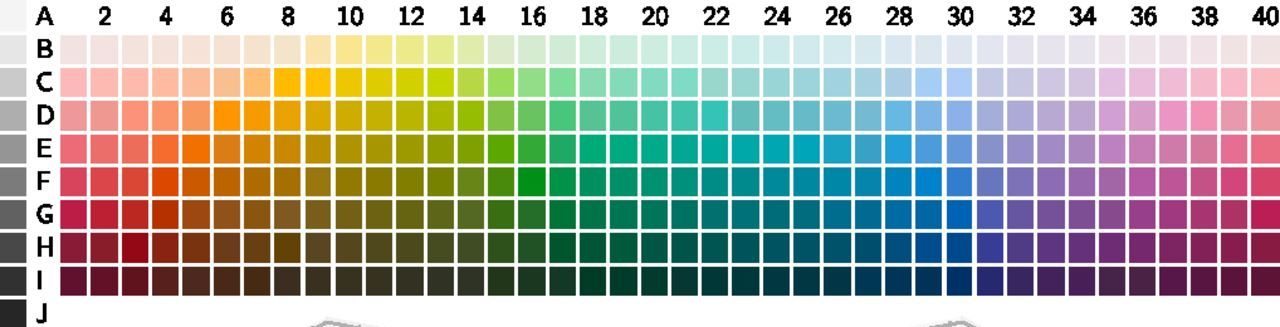
\includegraphics[width=0.49\textwidth]{docs/intro_rate_distortion/graphs/colour_palette.jpg}
    \caption{Colour palette introduced by \citet{berlin1991basic}}
    \label{fig:colour_palette}
\end{figure}

\subsection{Acquisition of Colour Terms}
\label{ssec:back_colour_learning}

Learning language starts from mapping concepts in words to objects and situations in our real world \cite{mollica2021logical}.
\citet{bleys2005colourcategory} first attempted to model the colour term acquisition as a multi-agent model, although they focus more on biases in the emergence of community-wide systems instead of the developmental trajectories of the learners.
\citet{beekhuizen2015perceptual} then proposes to model the problem following the Generalised Context Model \citep[GCM;][]{nosofsky1987attention}, and run simulation on the English data from \citet{bateman1915}.
To overcome the limitation of GCM on the ability to acquire language-specific attention weighting, \citet{beekhuizen2016modeling} then introduces Self-Organising Maps \cite{kohonen2001self} to further model the developmental and linguistic relativity effects in colour term acquisition.
While these works showed interesting results that match with the developmental data of children speaking different languages, none of them takes communicative efficiency into consideration during learning of colour terms.
However, in our case, we try to connect learning with communicative efficiency, and thus being an exploratory work, we chose a simple representation, i.e. the Gaussian models in \citet{zaslavsky2018efficient}. 
This will then serve as a good baseline and can be expended upon in future work using e.g. the methods mentioned above.

\subsection{Communicative Efficiency Modelling}
\label{ssec:back_colour_communicate}

Rate-distortion theory war originally proposed by \citet{shannon1959coding} to provide the theoretical foundations for lossy data compression. 
Human perception, e.g. visual and auditory sense, is also about extracting meanings from various noisy signals in the world, which suggests modelling perception under the rate-distortion framework \cite{sims2016rate}.
Regarding the colour naming problem, it can be thought as to compress information about a colour palette such as \cite{berlin1991basic} in to colour terms.
Therefore, \citet{zaslavsky2018efficient} proposed to model colour naming strategies in various languages under the rate-distortion framework, and showed that all languages achieve near-optimal strategies in the sense of compressing colours.
Further, they also showed that the partition of colours space across languages is soft rather than hard as assumed by previous works \citep[e.g.][]{levinson2000basic, maclaury1997color}, which supports us model the meaning of a colour term as a Gaussian distribution over all colours.
While there is vast literature on viewing language in information-theoretic perspective, \citep[e.g.][]{Piantadosi3526, gibson2013wordorder, levy2007speakers, Baddeley2009relation}, the existing works focus on how channel capacity effect syntactic structure.
In this work, we on the other hand study the semantics under rate-distortion framework, and we focus on the encoder itself instead of communication channels.

% \subsection{Modelling of Colour Naming}
\subsection{Our Modelling of Colour Naming}
\label{ssec:method_uni_components}

We use the colour chip palette introduced by \citet{berlin1991basic} as a way to encapsulate the colour domain.
The colour set $\mathcal{C}$ consists of $330$ chips $c$ that divide the colour space by luminosity and chroma.
We define a \textit{meaning} $m\in\mathcal{M}$ as a conditional distribution over colour chips, i.e. $p(c|m)$.
This meaning $m$ represents a colour that a speaker intends to convey.
Similarly to \citet{zaslavsky2018efficient}, we also define each meaning $m$ as a Gaussian distribution centred at a colour chip $\rc(m)$, i.e.
\begin{align}
    p(c|m)\propto \exp{-\frac{1}{\sigma^2}}||c-\rc(m)||^2
    \label{eq:p_c_given_m}
\end{align}
Following \citet{mokrzycki2011colour}, we use $\sigma^2=64$ to make colour chips distinguishable.

With a meaning from some cognitive source assumed to exist, we then define a \textbf{language} as a distribution of words conditioned on meanings --- $p(w|m)$ where $w$ denotes the words from a vocabulary.
A language is therefore the probability of emitting a word $w$ given a meaning $m$. \footnote{More details on the definitions of the random variables $m$, $c$ and $w$ can be found in Appendix~\ref{appssec:uni_components}.}

\section{Communicative Efficiency in Colours}
\label{ssec:method_comm}

Using our definitions of language and meaning in the colour space, we can link our approach to the classical communication model proposed by \citet{shannon1948mathematical} (Figure~\ref{fig:pipeline}).
Under this classical model, a speaker with an intended colour $m$ communicates a word $w$ to a listener who must then interpret it.

\begin{figure}[h]
    \centering
    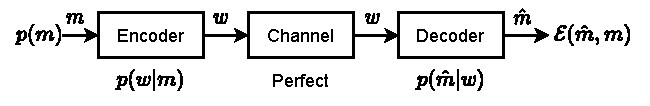
\includegraphics[width=0.49\textwidth]{graphs/cog_communication.pdf}
    \caption{
        A communicative model of colour naming.
        Note that the communication is about transmitting $m$ and reconstructing it as $\hat{m}$, thus there's no $c$ involved in the diagram.
    }
    \label{fig:pipeline}
\end{figure}

Communication starts from a cognitive source which specifies a distribution over meanings, $p(m)$. 
A speaker (\textit{encoder} in classical communication theory) samples a meaning $m~p(m)$, and encodes the meaning into a word following a language $p(w|m)$.
Since we focus on the semantic efficiency of languages, we assume a perfect communication channel that is noiseless --- the output of the channel is identical to its input.
After receiving a word $w$, a listener then interprets it as a meaning $\hat{m}$ following the listener's interpretation policy $p(\hat{m}|w)$.
\citet{zaslavsky2018efficient} proved that a Bayesian listener (decoder in Figure~\ref{fig:pipeline}) is an optimal interpretation policy if:
\begin{equation}
        p(\hat{m}|w) =
        \begin{cases}
            1 & \text{if $\hat{m}=w$}\\
            0 & \text{otherwise}
        \end{cases} 
        \label{eq:comm_listener}
    \end{equation}

Equation \ref{eq:comm_listener} implies that the mappings between $\hat{M}$ and $W$ are bijective, and that a listener would interpret different words as different meanings. %todo explain bijective?

% @todo rewrite this paragraph to make more sense
Intuitively, an ideal language should be as simple as possible while convey as much information as possible (intended meaning).
Under the above modelling of communication, an ideal language should minimise both its complexity (rate) and its information loss (distortion).
This trade-off between complexity and information loss forms the basis of rate distortion theory \citep[RDT,][]{shannon1959coding}.
Since we model all meanings (and therefore words) as distributions in the colour space, this trade-off can be formalised as an information bottleneck \citep[IB,][]{tishby2000information}.

% \subsubsection{Complexity of Language}
\subsection{Complexity of Language}
From an information-theoretic perspective, the complexity of a language $p(w|m)$ is defined as its information \emph{rate}, i.e. the mutual information between words $W$ and meanings $M$:
\begin{equation}
    I(M;W) = \sum_{m,w} p(m)p(w|m)\log \frac{p(w|m)}{p(w)}
    \label{eq:comm_complexity_definition}
\end{equation}
The minimum complexity is $0$ where the speaker refer to all colours with a single word. 
This matches with our intuition that the worst case is the language which conveys no information about the intended meaning of a speaker.

Given $p(m)$, the amount of information conveyed can be measured by its entropy $H(M)$, which can be further expanded as:
\begin{equation}
    H(M)=I(M;W)+H(M|W) 
\end{equation}
$I(M;W)$ is how many extra information about $m$ is conveyed by $w$, or the amount of information conveyed by the language.
Assuming that more information requires higher complexity, then the complexity of a language can be measured by $I(M;W)$, or at least, there should exist a positive correlation between complexity and $I(M;W)$.

% \subsubsection{Information Loss of Language}
\subsection{Information Loss of Language}
As shown in Figure~\ref{fig:pipeline}, the information loss (\emph{distortion} in RDT and IB) between a reconstructed meaning $\hat{m}$ and the original meaning $m$ is measured by an error function $\mathcal{E}(\hat{m}, m)$.
Since both $m$ and $\hat{m}$ are distributions over colour chips, we use the Kullback–Leibler (KL) divergence as our error function:
\begin{align}
    \mathcal{E}(m,\hat{m}) &\triangleq  D[m||\hat{m}] \label{eq:1}\\
    & = D[p(c|m)||p(c|\hat{m})]  \label{eq:2}\\
    % & = \sum_{c} q(c|\hat{m}) \log \frac{q(c|\hat{m})}{q(c|m)} \\
    & = \sum_{c} p(c|m) \log \frac{p(c|m)}{p(c|\hat{m})} \label{eq:3}\\
    & = \sum_{c} p(c|m) \log \frac{p(c|m)}{p(c|w)} \label{eq:4}
\end{align}
Where Equation~\ref{eq:4} is a result of our optimal interpretation policy (Equation~\ref{eq:comm_listener}). 

Given a language and an interpretation policy, we derive the joint distribution of $\hat{m}$ and $m$ as:
\begin{equation}
    \begin{split}
        p(\hat{m},m) 
        & = p(\hat{m}|m)p(m) \\
        & = \sum_w p(\hat{m}|w)p(w|m)p(m)
    \end{split}
    \label{eq:joint_c_hat_c}
\end{equation}

Then, for a language, information loss can be defined as the expectation of error over the joint distribution:
\begin{equation}
    \begin{split}
        & \mathbb{E}_{p(\hat{m},m)}\left[D[m||\hat{m}]\right] \\
        & = I(M;C) - I(W;C)
    \end{split}
    \label{eq:comm_info_loss}
\end{equation}
Since $I(M;C)$ is independent of $p(w|m)$, we can minimise $-I(W;C)$ to reduce the expected distortion.\footnote{The full derivation of Equation~\ref{eq:comm_info_loss} can be found in Appendix~\ref{appssec:derivation_of_info_loss}.}

\subsection{The Information Bottleneck Method}

To obtain the optimal languages that balance complexity and information loss, we optimise the following IB objective function:
\begin{equation}
    \mathcal{F}[p(w|m)] = I(M;W) - \beta I(W;C)
    \label{eq:comm_IB_objective}
\end{equation}
Where $I(M;W)$ corresponds to complexity, $-I(W;C)$ corresponds to information loss, and $\beta$ is a hyper-parameter for balancing the trade-off.

To minimise the IB objective, we use the Blahut-Arimoto algorithm \citep{arimoto1972algorithm, blahut1972computation} to optimise $p(m)$ and $p(w|m)$ iteratively.
This is possible because they have the same concavity.
Therefore, by solving the optimisation problem, we can find an optimal $p(m)$ (the cognitive source of meanings) and optimal languages $p(w|m)$ at the same time.

% TODO: double check that this is right ..
\begin{algorithm}[h]
    \SetAlgoLined
    \SetAlgorithmName{Algorithm} \\
    \KwInput{\textbf{Input}: $\mathcal{D}$, $\beta$} \\
    % Set an IB objective with $\beta$; \\
    
    % Minimise IB objective by optimising $p(w|m)$ and $p(m)$; \\
    % Record complexity $I(M;W)$ and information loss $-I(W;C)$ \\
    % \KwIn{\textbf{Input:} $\mathcal{D}$, $\mathcal{N}$} \\
    % Fit adult model $P(M|\mathcal{D})$ \\
    % $\mathcal{D}' \gets \varnothing$ \\
    Calculate $p(w,m)$ prior from $\mathcal{D}$ \\
    Initialise $p(m|w)_0$ as identity matrix $I$ \\
    \For{$\beta_i \in \beta$}{
        Calculate optimal $p(m|w)_i$ using Blahut-Arimoto($\beta_i$, $p(w,m)$, $p(m|w)_0$) \\
        % Sample $\mathcal{S} \sim P(M|D)$ such that $|S \cup D'|=N$ \\
        % $\mathcal{D}' \gets S \cup D'$ \\
        Record complexity $I(M;W)$ and information loss $-I(W;C)$ for $p(m|w)_i$ \\
        % $r_i$, $d_i$ $=$ score($q_i$, $p(w,m)$) \\
        % Fit child model $P(H|D')$ \\
        % Record complexity $I(H;C)$ and information loss $D[(M|\mathcal{D})||P(H|\mathcal{D}')]$
    }
 \caption{Calculating the optimal complexity and information loss (rate and distortion) in the communicative efficiency problem.}
 \label{al:comm_algo}
\end{algorithm}

The final method to compute the rate and distortion under the communicative efficiency approach is shown by Algorithm~\ref{al:comm_algo}.
Where typically a dataset $\mathcal{D}$ would be used to calculate priors $p(w|m)$, here we initialise $p(w|m)$ to the Identity matrix and use the Blahut-Arimoto algorithm to optimise it given a range of $\beta$ values.
% Several $\beta$ values are taken from a wide range to optimise over
For each $\beta_i$, we find a theoretically optimal language $p(w|m)$ that satisfies the objective of minimising complexity and information loss.


\section{Learning Colours}
\label{ssec:learning}

%To better illustrate the learning problem, we visualise it as a directed acyclic graph shown in Figure~\ref{fig:pipeline_dag}.
In the learning problem, our task is to infer the posterior probability $P(M|\mathcal{D})$ given a data set $\mathcal{D}$ consisting of word and colour chip pairs, i.e. $\mathcal{D}=\left\{w_n, c_n\right\}_{n=1}^{N}$. %What is M? 
We call such a model an \textit{adult model}, as it corresponds to the model an adult speaker could have learnt when exposed to all of the available data. %TODO: Any reference or more accurate justification for this last statement?

However, we are primarily interested in understanding the role of learnability on the development of colour term acquisition. 
\textcolor{red}{Define learnability.} 
Inspired by children's apparent preference to learn simpler models first~\cite{tenenbaum2020hacker}, we study learnability by learning and comparing hypothetical models of meanings on increasing amounts of data. 
We use $H$ to indicate the set of hypothetical meanings, though mathematically $H$ has the same type and domain as $M$. 
Analogously to $P(M|\mathcal{D})$, we call a learnt model of hypothetical meanings $P(H|\mathcal{D}')$ a \textit{child model}, as this corresponds to a model a child with limited amounts of data could have learnt.

%starting from the simplest possible model where every colour is assigned the same term.

% \begin{figure}[h]
%     \centering
%     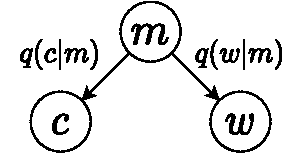
\includegraphics[width=0.4\textwidth]{docs/intro_rate_distortion/graphs/cog_comm_dag.pdf}
%     \caption{Illustration of learning problem in a DAG.}
%     \label{fig:pipeline_dag}
% \end{figure}

\subsection{Optimisation Objective}
\label{sssec:learn_optim}

Formally, the goal of the learning problem is to find a model that maximises the posterior as given by $P(H|\mathcal{D'})$. 
By applying Bayes' Rule, we obtain the following derivation:
\begin{equation}
    \label{eq:learning_objective_pH_D}
    \begin{split}
        p(H|\mathcal{D'})
        & \propto p(\mathcal{D'}|H)p(H) \\
        & = \prod_{n=1}^{N} p(w_n, c_n|H)p(H)
    \end{split}
\end{equation}

To calculate this objective, we make the simplifying assumption that mappings between $H$ and $W$ are one-to-one. 
This allows us to work with the known and finite space of colour terms instead of the potentially infinite space of all possible hypotheses.
Thus, we can also factorise the joint probability as $p(w,c|h) = p(c|w)p(w|h)$.
%TODO: Citation for why we can make this one-to-one assumption?
% \begin{equation}
%     \begin{aligned}
%      & p(w, c|H) = p(c|w)p(w|h) \\
%     %  & =
%     %     \begin{cases}
%     %         p(c|w) & \text{if $h=w$}\\
%     %         0 & \text{otherwise}
%     %     \end{cases} 
%     \end{aligned}
%     \label{eq:factorise_data_pair}
% \end{equation}

Following our settings in the communication problem, we model $p(c|w)$ as a Gaussian distribution centred at some $\rc(w)$ with covariance $\Sigma(w)$. 
The likelihood in Equation~\ref{eq:learning_objective_pH_D} is then maximised by calculating the sample mean and covariance of colour chips $c_n$ that appear together with the colour term $w_n=w$.

Finally, we model the distribution of words $p(w|h)$ with a categorical distribution whose parameter is the vector of normalised word frequencies calculated from the data.
 
% Furthermore, we define the prior over hypotheses $p(H)$ to prefer simpler models over more complex ones, following previously observed behaviour of children~\cite{todo}. \textcolor{orange}{@Coleman: Could you add a description of how the simplicity prior is calculated?}
% \subsection{A simplicity prior for colour systems}
% \label{ssec:simplicty_prior}
% What colour systems should be considered a priori more likely?
% We operationalise the notion of the \textit{simplicity} of a hypothesized colour system. 
% We have operationalised words in a colour system as being multivariate normal distributions in the 3-dimensional CIELAB space. 
% Intuitively, a simple colour system to learn is one in which 1. there are few words 2. words have minimal overlap. 
% To compute the overlap between words, we use the Bhattacharyya coefficient~\cite{fukunaga1990stats}. 
% This is a measure between 0 and 1 for the overlap of two probability distributions $p$ and $q$. 
% In its general form, it is given by
% \begin{align}
%     BC(p,q)=\int\sqrt{p(x)q(x)}\,dx
% \end{align}
% For the special case in which $p$ and $q$ are both multivariate Gaussians (as is the case here), the Bhattacharyya coefficient is given by
% \begin{align}
%     \exp(\frac{1}{8}(\mathbf{\mu}_1-\mathbf{\mu}_2)^{\top}\mathbf{\Sigma}^{-1}(\mathbf{\mu}_1-\mathbf{\mu}_2)\exp(
% \end{align}


% \subsubsection{Measuring Learnability}\label{sssec:learnability}
\subsection{Measuring Learnability}\label{sssec:learnability}
% The complexity of a language in the learning problem is given by the mutual information $I(W;C)$ between $W$ and $C$. Factoring in our definition of a simplicity prior, we have the full joint $p(w,c,h)=p(c|w)p(w|h)p(h)$ and the mutual information which is then calculated as follows:
% \begin{align}
% \sum_{w,c} p(w,c,h)\log\frac{p(w,c,h)}{p(w,h)p(c,h)}
% \end{align}
% Where the terms in the denominator are marginal distributions. This definition provides a way to measure the amount of information conveyed by the hypothetical language about the colour space. 

The complexity of a language in the learning problem is given by the mutual information $I(W;C)$ between $W$ and $C$. Using that the joint is $p(w,c|h)=p(c|w)p(w|h)$ the mutual information which is calculated as follows:
\begin{align}
\sum_{w,c} p(c|w)p(w|h)\log\frac{p(c|w)}{p(c|h)}
\end{align}
Where the term in the denominator is a marginal distribution from the joint. This definition provides a way to measure the amount of information conveyed by the hypothetical language about the colour space. 

% The prior colour-chip distribution $p(C)$ is given by the least informative prior as described in~\cite{zaslavsky2018efficient}. This formulation is equivalent to mixising the mutual information $I_q(W;C)$ and can be evaluated using the Blahut-Arimoto algorithm. We call this prior the least informative prior because it maximises the expected KL-divergence between prior and posterior:

% \begin{align*}
%     % \begin{split}
%         & I_q(W;C)\\
%         &  = \sum_{w,c} p(w)p(c|w)\log \frac{p(c|w)}{p(c)} \\
%         &  = \sum_{w} p(w) \sum_c p(c|w)\log \frac{p(c|w)}{p(c)} \\
%         &  = \sum_{w} p(w) D[p(c|w)||p(c)] \\
%         & = \mathbb{E}_{W}[D[p(c|w)||p(c)]
%     % \end{split}
%     \label{eq:least_informative_prior}
% \end{align*}

% A prior distribution is calculated over all real-world languages following the formulation:

% \[p(C)=\argmax_{p(C)} H(C)-H_q(C|W)\]

% That is, we aim to maximise the uncertainty about our prior colour distribution while minimising the expected uncertainty of $c$ given $w$. Here $H_q(C|W)=-\sum_{c,w} p(c)p(w|c)\log \frac{p(c|w)}{p(c)}$ is the conditional entropy. 

Information loss in the learning problem follows from the approach that child models are trained on a subset of the data sampled from the adult model and therefore cannot encode more information than the adult model. 
The exact information-loss is then measured as the KL-divergence of the child model from the adult model given by $D[P(M|\mathcal{D})||P(H|\mathcal{D}')]$.

Our method for generating hypothetical languages then mimics the children's learning process~\cite{mollica2021logical} and proceeds as follows. 
We iteratively accumulate a data set by adding samples drawn from the adult model. 
On each iteration, we train a new child model on this increasingly larger data SET. 
The child model is then evaluated according to the measures defined above and the scores are recorded. 
Finally, we can show how the child models learn as they are exposed to more data by plotting the measured complexities against the information-losses. 

This entire procedure is summarised in Algorithm~\ref{al:learn_algo}. We vary the number of samples $N$ from the set $\mathcal{N}$ containing sample sizes from $1$ to $100K$ with lower numbers sampled more densely than higher numbers.

\begin{algorithm}
    \SetAlgoLined
    \SetAlgorithmName{Algorithm} \\
    \KwIn{\textbf{Input:} $\mathcal{D}$, $\mathcal{N}$} \\
    Fit adult model $P(M|\mathcal{D})$ \\
    $\mathcal{D}' \gets \varnothing$ \\
    \For{$N \in \mathcal{N}$}{
        Sample $\mathcal{S} \sim P(M|D)$ such that $|S \cup D'|=N$ \\
        $\mathcal{D}' \gets S \cup D'$ \\
        Fit child model $P(H|D')$ \\
        Record complexity $I(H;C)$ and information loss $D[(M|\mathcal{D})||P(H|\mathcal{D}')]$
    }
 \caption{Calculate complexity and information loss in the learning problem.}
 \label{al:learn_algo}
\end{algorithm}




% \subsubsection{Trade-off Implied by Maximising the Posterior}
\subsection{Trade-off Implied by Maximising the Posterior}
\label{sssec:learn_tradeoff}

% Since the logarithm is a monotonic function, the maximum of $P(H|\mathcal{D})$ is also the maximum of $\log P(H|\mathcal{D})$. Therefore, to maximise Equation~\ref{eq:learning_objective_pH_D}, it's the same to maximise the following log-likelihood of hypothesis $H$:

By choosing to optimise the posterior distribution, we can draw a parallel to the IB method of the communication problem in Section~\ref{ssec:method_comm}. 
Since the logarithm is a monotonic function, for optimisation we can consider the decomposition of the log-posterior:
\begin{align*}
    % \begin{split}
        & \log p(H|\mathcal{D'}) \propto \log \prod_{n=1}^{N} p(w_n, c_n|H)p(H) \\
        &  =\sum_{n=1}^{N} \log p(H) p(w_n, c_n|H) \\
        % &  =\sum_{n=1}^{N} \log p(H) \log p(w_n, c_n|H) \\
        % &  =\underbrace{N\log p(H)}_{\text{constant, simplicity}} + \underbrace{\sum_{n=1}^{N} \log p(w_n, c_n|H)}_{\text{variable, information loss}} \\
        &  =N\cdot\underbrace{\log p(H)}_{\text{constant}} + \underbrace{\sum_{n=1}^{N} \log p(w_n, c_n|H)}_{\text{variable}} \\
    % \end{split}
    \label{eq:learning_objective_log_pH_D}
\end{align*}

% Note that in the above equation, it consists of two terms: 1) $\log p(H)$ which is a constant; 2) $\sum_{n=1}^{N} \log p(w_n, c_n|H)$ is a variable.
We can view the number of samples $N$ to play a similar role to the $\beta$ hyper-parameter in the IB method. 
If $N$ is very small, then the log-likelihood $\log p(H|\mathcal{D}')$ would dominate, which is mathematically an alternative measure of information loss (see Appendix~\ref{appssec:ll_learning_loss}).
Otherwise, $p(H)$ dominates which corresponds to the a priori complexity of our hypothesis.



% \subsubsection{Complexity of Hypotheses}
% \label{ssec:learn_complexity}

% After solving the estimation problem illustrated in Section~\ref{ssec:learn_optim}, for each $h\in\mathcal{H}$, we will have a corresponding mode $\rc(h)$, and variance $\Sigma(h)$. 
% At the same time, we will also have a mixing coefficient $\pi_n$ for every $c_n$ in the dataset.
% Therefore, we can easily calculate the mutual information between $H$ and $C$ as follow:
% \begin{equation}
%     I(H;C) = \sum_{h,c} p(c|h)p(h)\log\frac{p(c|h)}{p(c)}
% \end{equation}

% simulate actual kid learning
% use schedule m
% calculate likelihood over all the color chips and average, multiply by N to get number of data points
% that is beta for tradeoff

% p(H) dirichlet process prior -- favor as few lumps (gaussians) as possible
% penalize the gaussian prior on how close the means and std dev
% 8 terms in english, 8 gaussians, reward gaussians that are basically the same thing
% reward gaussian with similar means
% reward wider std deviation


% ideally variational/dirichlet

% generate hypotheses with a schedule, each hypotheses get n data points on the schedule
% oversample lower end

% information loss not on training data but on WCS data (uniform)

% multiply the plot (information loss) by N the number of data points for the hypothesis (dont)

% or just plot at N=1 :D

% \section{Experiment}
% \label{sec:experiment}



\section{Experiments}
\label{sec:experiments}

In this section, we present our experiments and their results. First, we describe separate experiments using the methods from the communicative efficiency and the learning problem. We then join the two problems and present our main results on the interaction of the problems. Throughout this section, we highlight for presentation the same languages (Agarabi, Culina, Dyimini, Yucuna) in our results, following the choices of \citet{zaslavsky2018efficient} but replacing English with Yucuna.
% Once we have the complexity and information loss values in both problems for a pair of $(\beta, N)$, we can plot one point in the communication curve like shown in Figure~\ref{fig:curve_comm}, and another point in the learning curve.

\subsection{Communicative Efficiency}

\begin{figure}
    \centering
    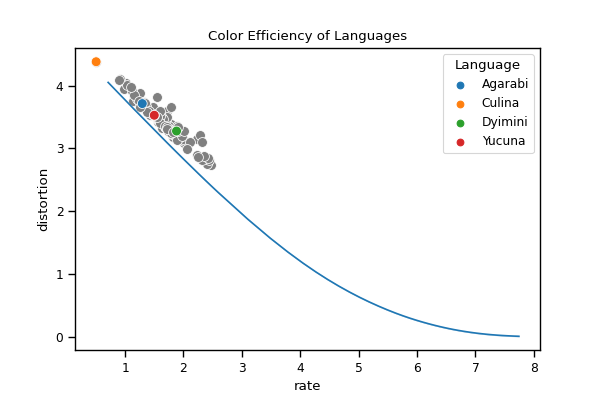
\includegraphics[width=0.5\textwidth]{docs/final_report_for_course/graphs/color_efficiency.png}
    \caption{The communicative efficiency of real languages plots along the frontier.}
    \label{fig:communicative_efficiency}
\end{figure}

We first score the different languages of the WCS in relation to the rate distortion frontier in Figure~\ref{fig:communicative_efficiency}.
The frontier (blue line) is calculated using the Blahut-Arimoto algorithm and varying values of the trade-off parameter $\beta$.
Any point on the frontier describes an optimal language for a given hyper-parameter $\beta_i$.

We score each language according by calculating the $p(w|m)$ from their collected samples in the WCS.
As in \citet{zaslavsky2018efficient}, we find that real languages are distributed along the frontier.
This indicates that human language tend to approach the frontier and embody the trade-off between complexity and information loss.

However, Figure~\ref{fig:communicative_efficiency} also shows that certain real languages such as Culina, an Arawan language from Brazil and Peru, appear at different points on the frontier than others.
As \citet{zaslavsky2018efficient} also , Culina stands out because it does not distribute the colour space in approximately the same ways as most other languages.
In particular, it does not have a `basic' distinct word for the English colour green.
With a particular emphasis on `basic' because the WCS dataset only includes colour words which are only generally used in the context of colour.
Because the score of rate/distortion for each language is evaluated using a universal prior over all languages, if a language is very different from others then this will be reflected in where the language is scored. 


\subsection{Learnability}
\label{ssec:results_learning}

\begin{figure}
    \centering
    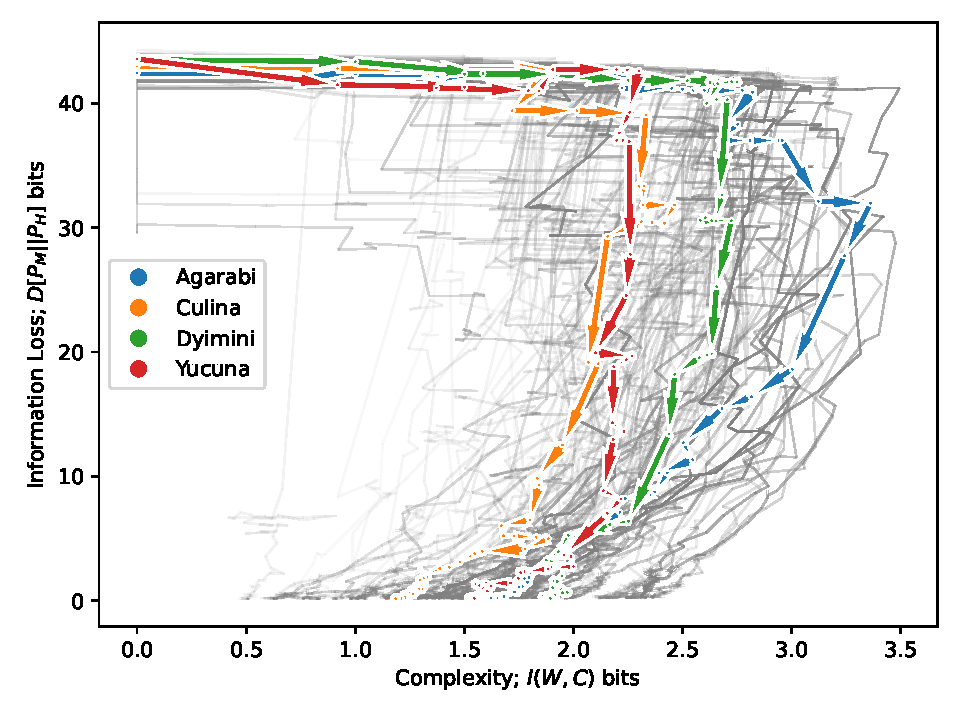
\includegraphics[width=0.5\textwidth]{docs/final_report_for_course/graphs/cplx_inf_loss.pdf}
    \caption{Learning trajectories of child models plotted in the complexity-information-loss space. Each grey line shows the evolution of one language with the line thickness being the number of colour terms in the adult model.}
    \label{fig:learn_infloss_complex}
\end{figure}

The main results of Algorithm~\ref{al:learn_algo} can be seen in Figure~\ref{fig:learn_infloss_complex}.
 
 \begin{figure}
     \centering
     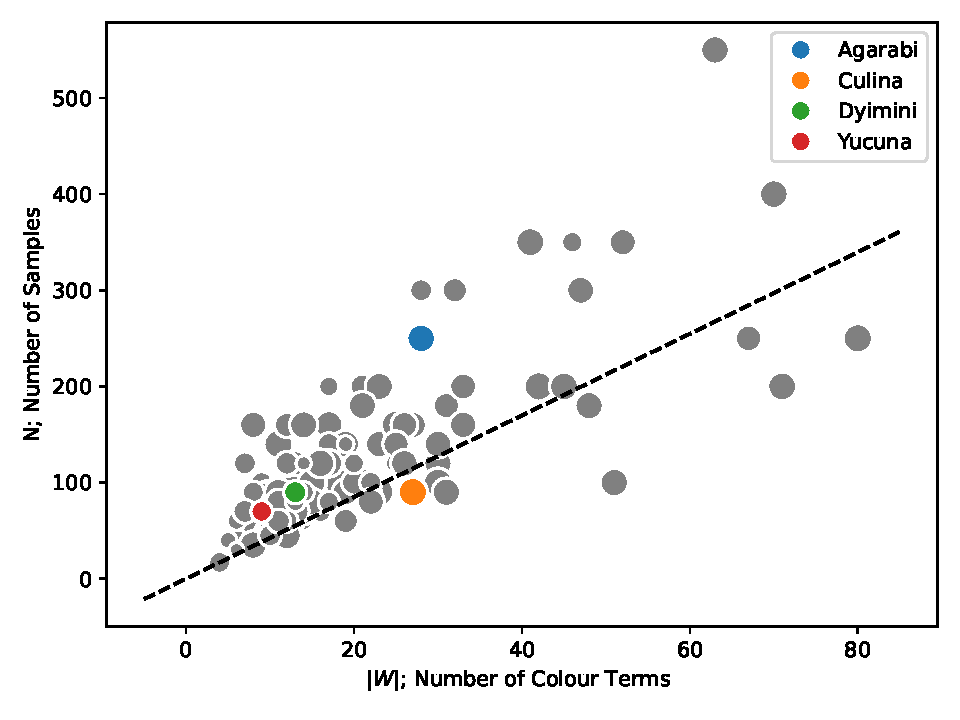
\includegraphics[width=0.5\textwidth]{docs/final_report_for_course/graphs/nw_samples.pdf}
     \caption{Number of samples needed to reach an information-loss less than 5 bits as a function of the number of words in the language. Marker sizes are proportional to the actual information-loss at the given sample count.}
     \label{fig:nw_samples}
 \end{figure}
 
\subsection{Effects of $\mathcal{N}$ on Communicative Efficiency}


\begin{figure}
    \centering
    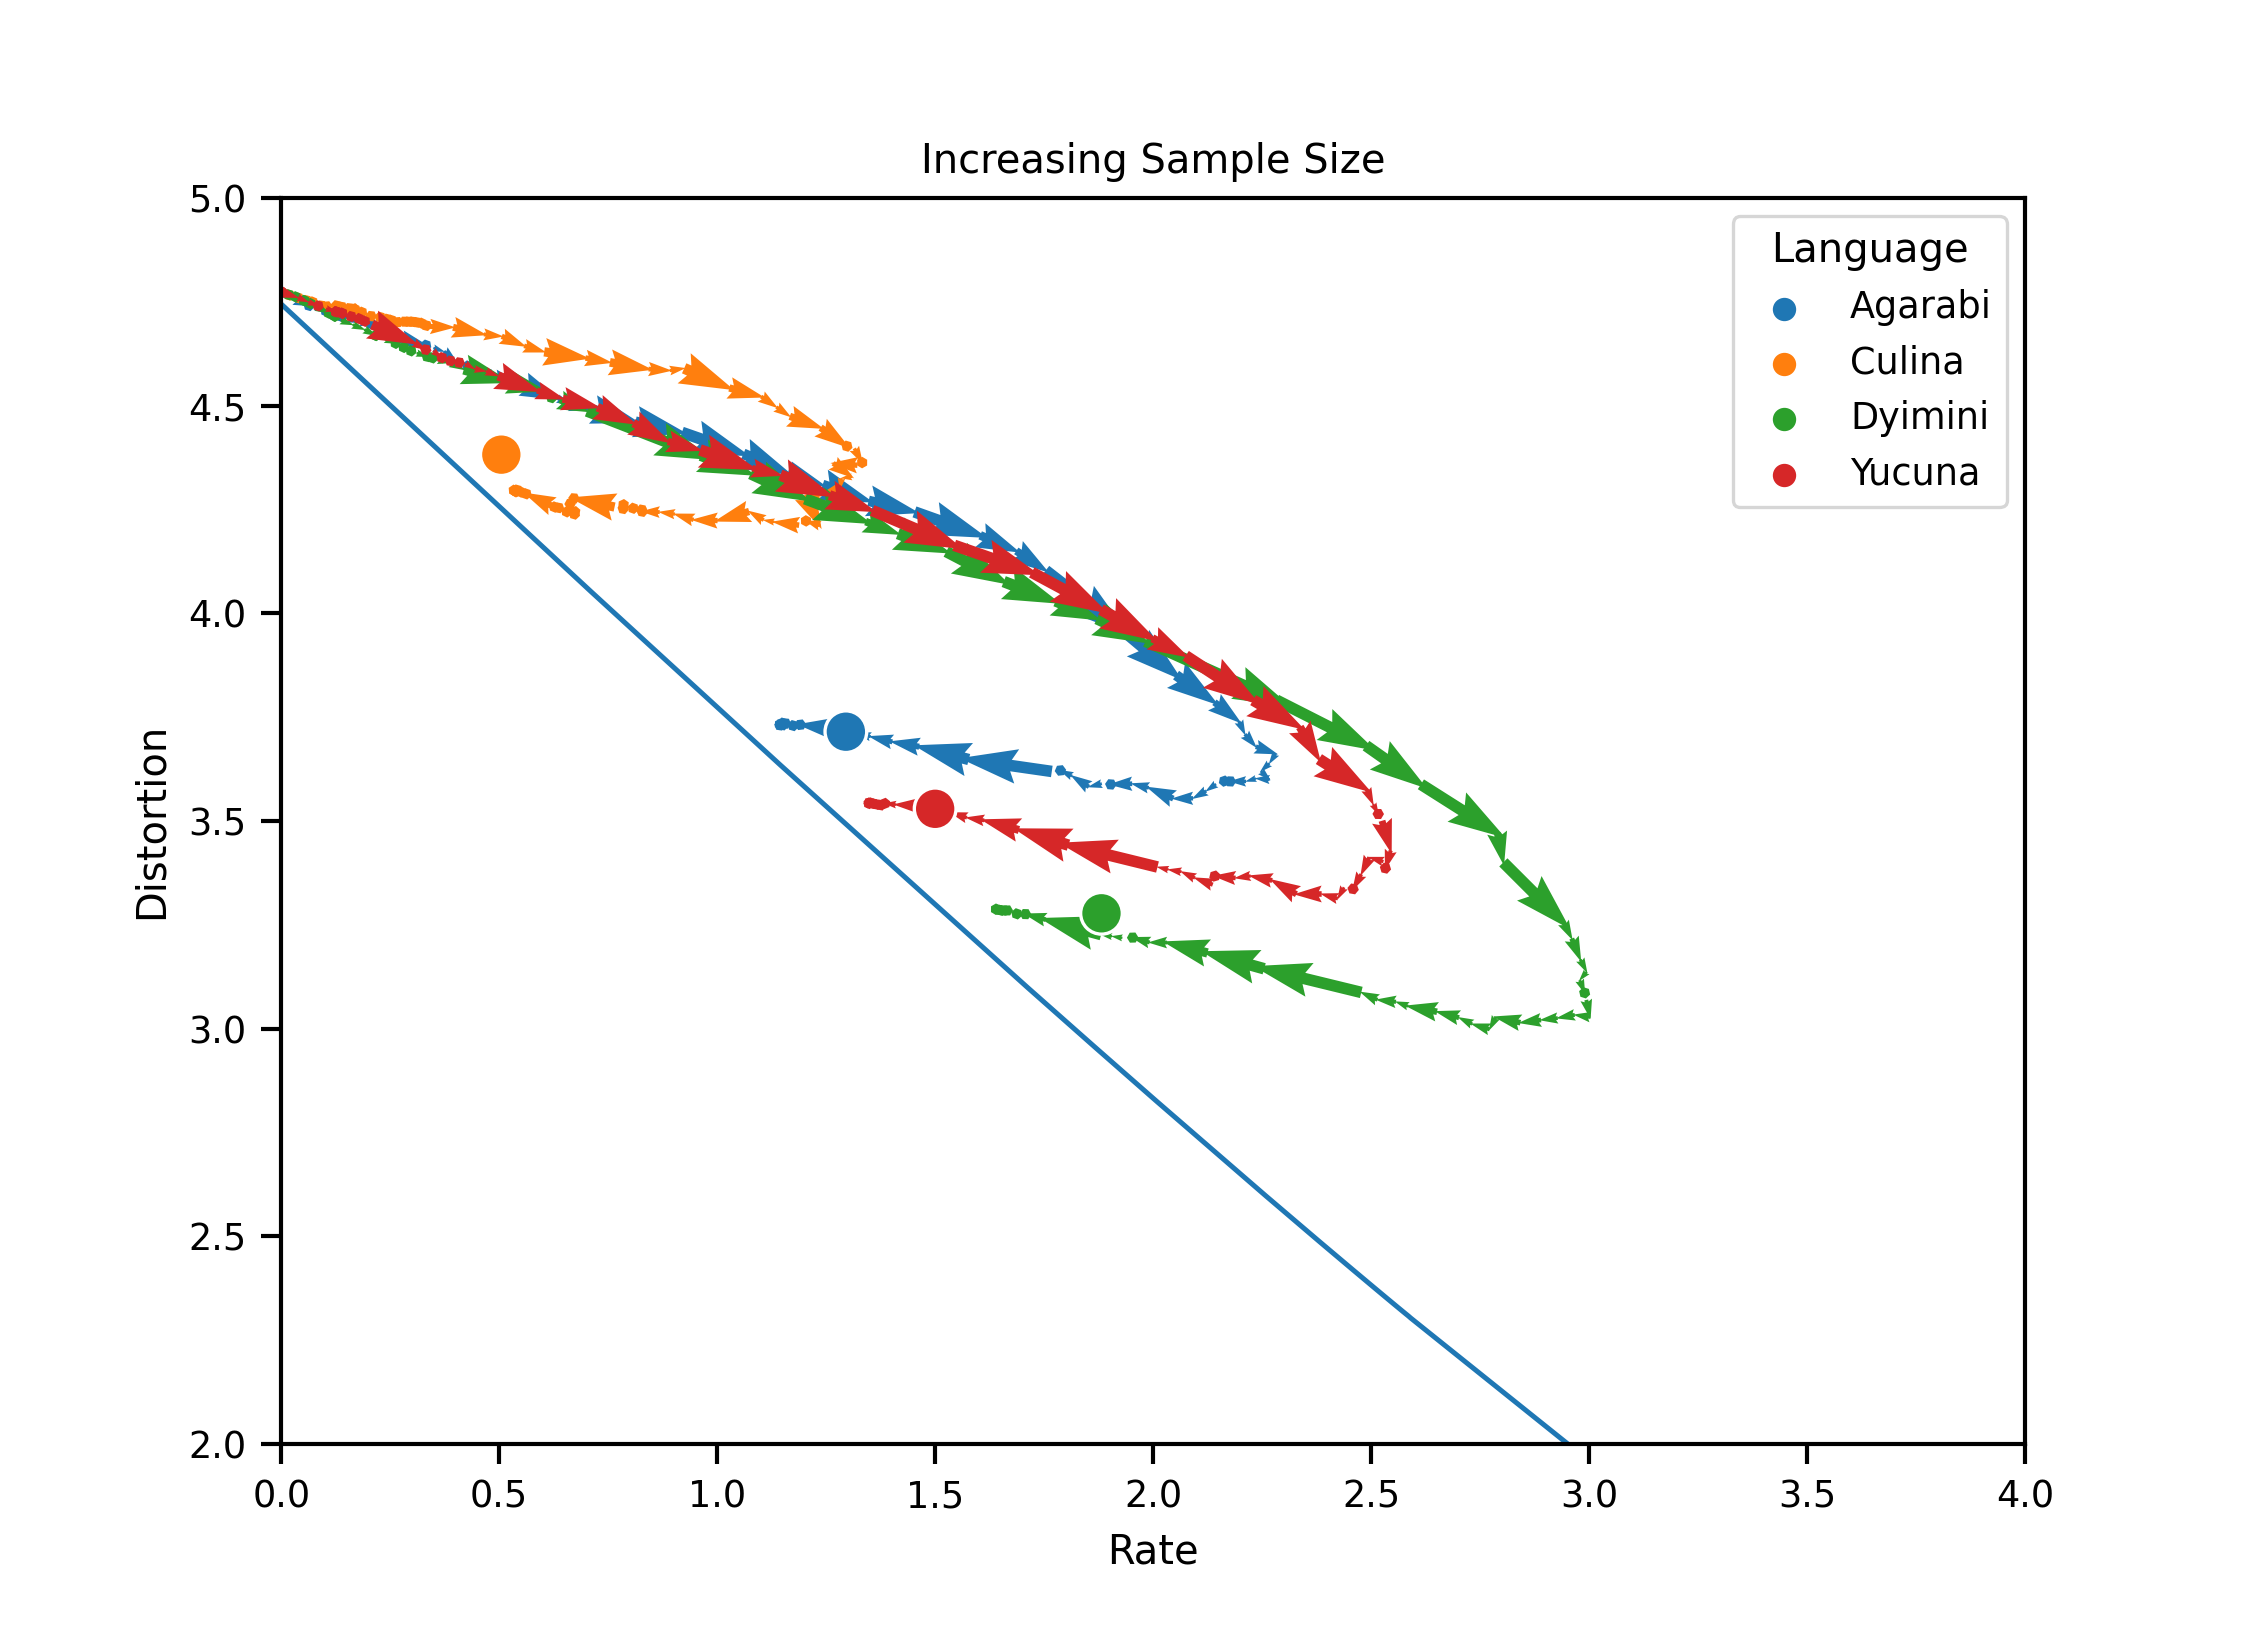
\includegraphics[width=0.5\textwidth]{docs/final_report_for_course/graphs/comm_sample_increase.png}
    \caption{The dynamic relationship between Rate and Distortion as sample size increases is plotted in relation to the frontier.}
    \label{fig:comm_sample_increase}
\end{figure}

Using the sampled datasets $\mathcal{D}$ from varying $\mathcal{N}$ with our adult model, we can score the communicative efficiency of the language as more data points are added over time.
Figure~\ref{fig:comm_sample_increase} shows the trajectory of rate/distortion for a given language as we increase the number of samples $\mathcal{N}$.
We observe that the rate and distortion do not change at the same rate as the frontier as we increase the number of samples.
With a single sample, the language has a high distortion but a low rate --- it is not informative but simple. 
As more samples are added this reduces the distortion and increases the rate, as more words are added the complexity rises but the information increases with it.

Interestingly Figure~\ref{fig:comm_sample_increase} shows that after a certain point, the dynamic reverses and the rate starts decreasing as distortion increases. 
As more samples are added and the colour space is covered by $\mathcal{D}$, the probabilities are smoothed and the language as a whole is simpler (lower rate) albeit with slightly more information loss (higher distortion).
But the overall slope of the dynamic is different, and with more samples, languages slowly re-approach the frontier except at a higher rate.

The real language scores in Figure~\ref{fig:comm_sample_increase} are indicated by their respective points.
It is important to note that because we are sampling from the adult model, the trajectories terminate exactly at the real language score.
This is because the sampling operation is approximate and can be allowed to over-sample examples in the original dataset.


\begin{figure}[h]
    \centering
    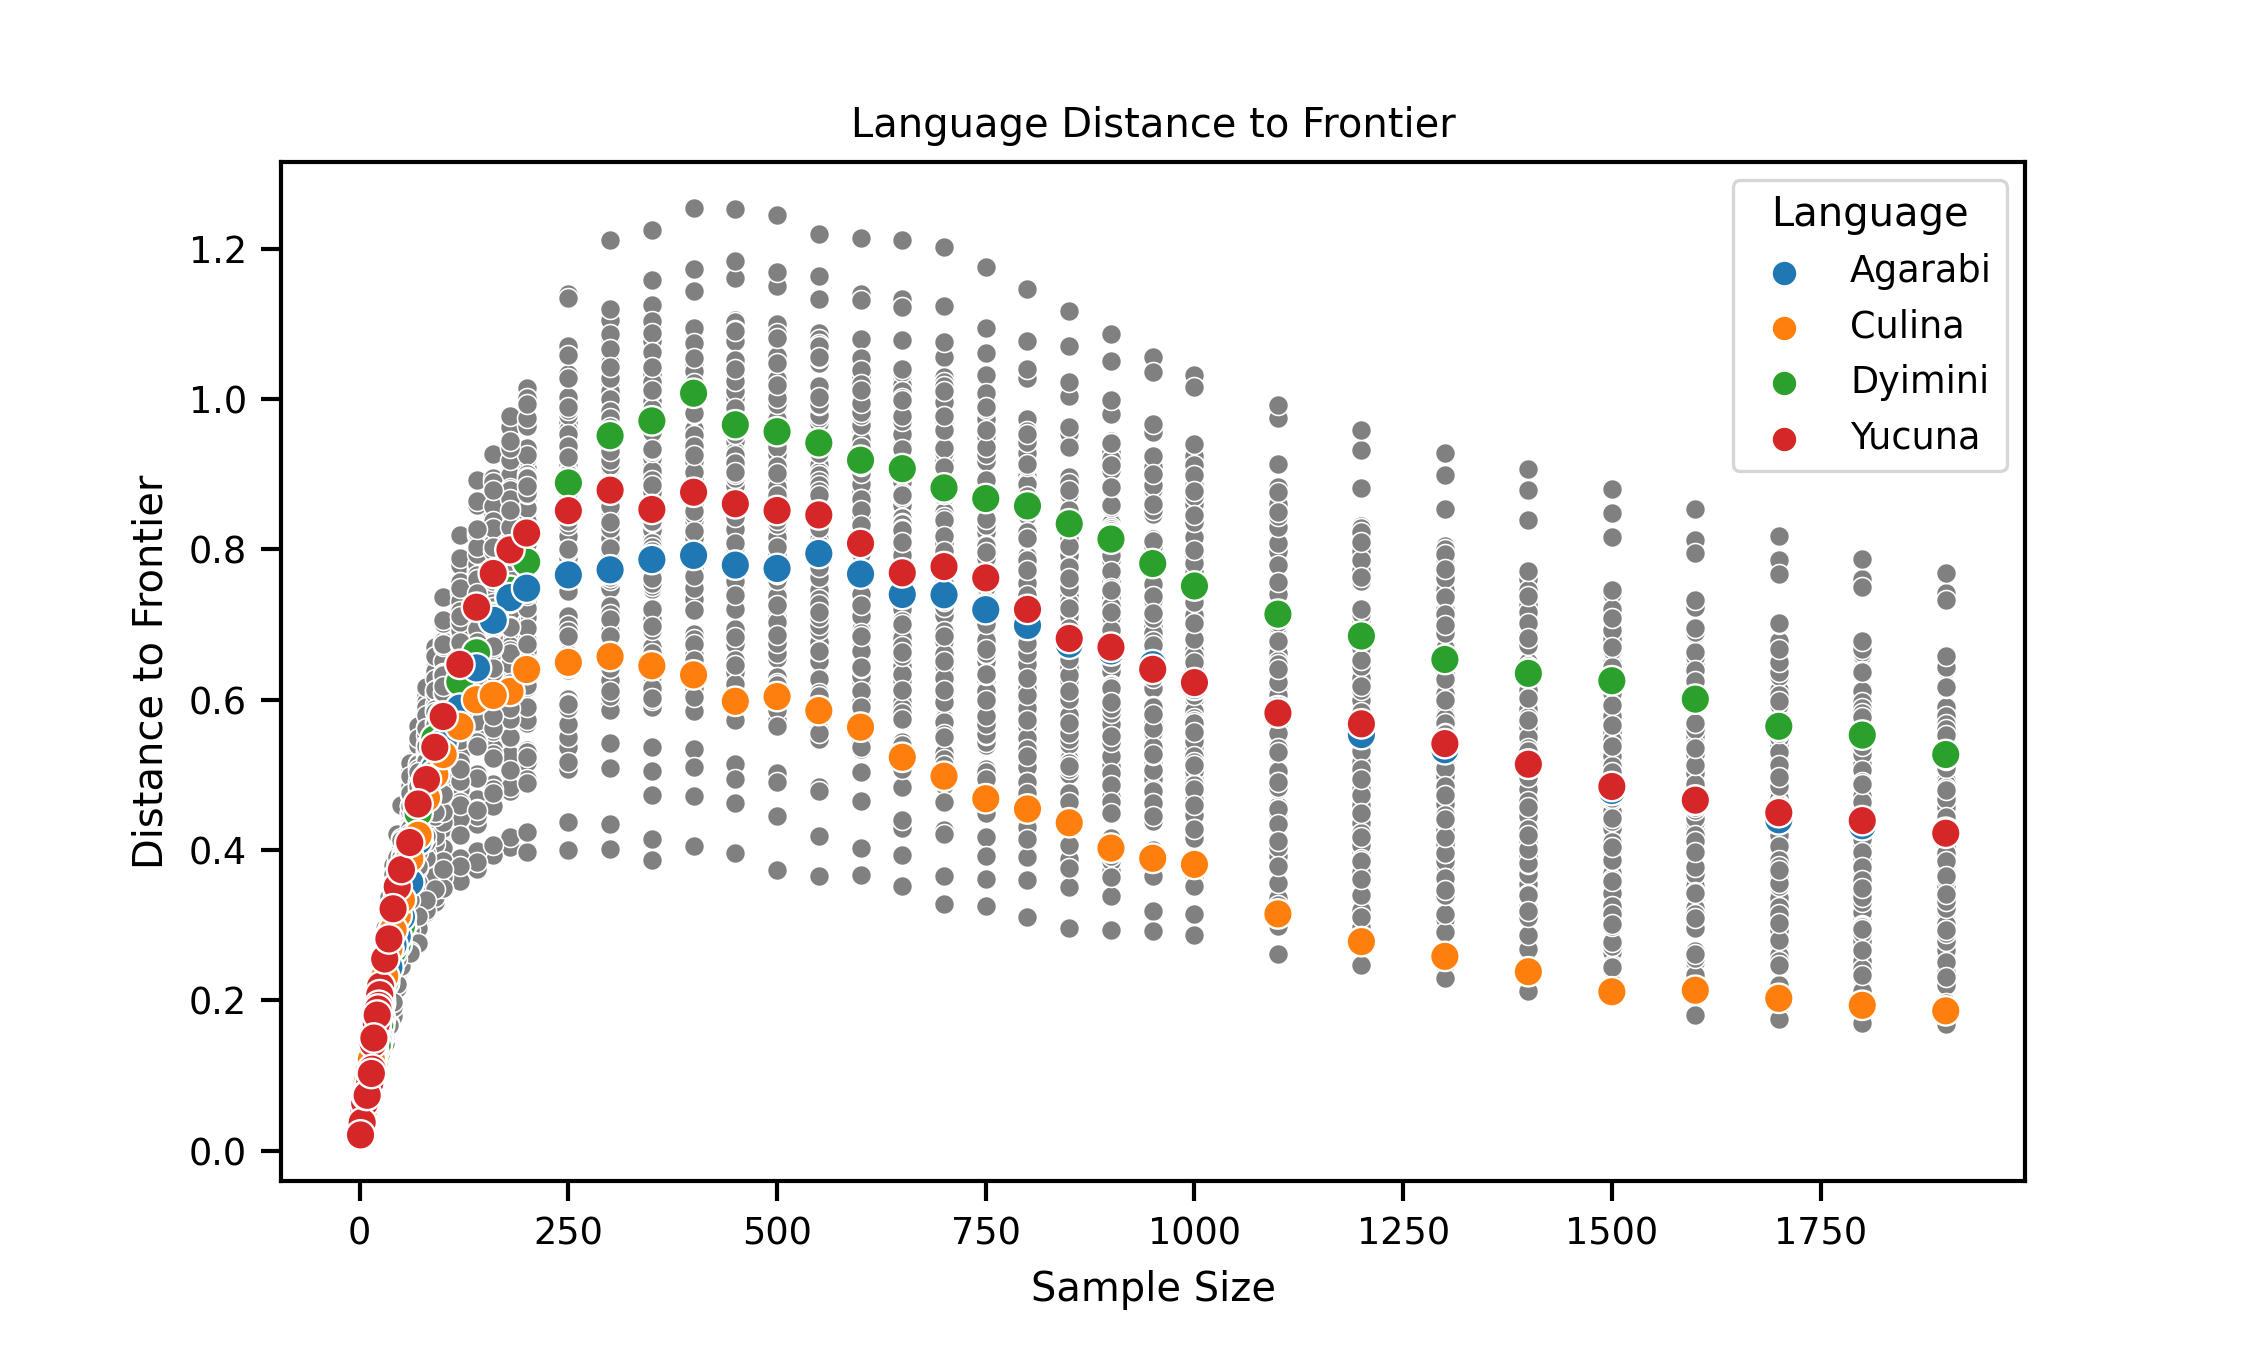
\includegraphics[width=0.5\textwidth]{docs/final_report_for_course/graphs/dist_frontier.png}
    \caption{The distance to frontier for each language first increases with $N$ and then decreases.}
    \label{fig:dist_frontier}
\end{figure}


Figure~\ref{fig:dist_frontier} shows the distance of a language sample to a frontier given its sample size.
Again, we observe that the dynamic reverses after a certain point and the distance to the frontier starts decreasing as more samples are added.
This follows the same trend across all 110 languages, where the curve back towards the frontier can be observed as more data points are sampled.

% - Plot distance to frontier over N from 
% -> Express more and more and things and rate d


\section{Discussion}

As a results of our experiments we find that developmental constraints are ?not? active in the communicative efficiency trade-off. 
The dynamic that occurs in Figure~\ref{fig:comm_sample_increase} and Figure~\ref{fig:dist_frontier} result from the fact that the developmental model is not following the pareto frontier.
Thus we believe that both models, learnability and communication efficiency, should indeed be treated as different mechanisms. 
Though it is important to note that Figure~\ref{fig:comm_sample_increase} and Figure~\ref{fig:dist_frontier}  also show complicated dynamics between learnability and communication efficiency, and so we can neither conclude that both are independent. 


% Developmental constraints -> active or not active? 


% fact that it's not following pareto frontier means that they are different things and affect dynamics 
% Complicated dynamics between learnability and communicative

%FUTURE WORK:
%Do CE -> Learn not just Learn -> CE
%Better learning method
%Fully Bayesian approach

\section{Conclusion}

From our observations in \ref{sec:experiments}, we initially find, similarly to \cite{zaslavsky2018efficient}, that real languages fall close to the Pareto frontier that describes the trade-off between complexity and information loss.
that the two approaches are
Future work will 

We conclude that communicative efficiency and learnability in development constitute separate, active constraints on the world's colour systems.


\section{Individual Contributions}
%  note explaining individual contributions
Overall we split the project into two groups of two, where Coleman and Balint led the development on the Learnability side, and Shangmin and Gautier led the Communication Efficiency side. 
Our individual contributions are listed below:

\begin{itemize}
    \item Coleman Haley: design of the Learnability prior, introduction and motivation,  ...
    \item Shangmin Guo: Background and Approach --- framing of the problem through math derivations and proofs, obtaining the frontier values,  ...
    \item Balint Gyevnar: design of the Learnability models and experiments ...
    \item Gautier Dagan: dealing with the WCS, bridging the Learnability with Communication Model, running the communication experiments, plotting and analysis ...
\end{itemize}

\bibliographystyle{acl_natbib}
\bibliography{main}

\newpage
\appendix

\section{More Details about the Modelling of Colour Naming}
\label{appsec:more_details}

\subsection{Random Variables Involved in Colour Naming}
\label{appssec:uni_components}

The variables involved in this project are listed as follows:
\begin{itemize}[leftmargin=*]
    \item \textbf{meaning $M$\footnote{In this document, a random variable is notated by a capital letter, e.g. $M$ here, its possible values are notated by the corresponding lower case letter, e.g. $m$, and the set of its sample space is notated by the corresponding calligraphic capital letter, e.g. $\mathcal{M}$.}}: a meaning $m\in\mathcal{M}$ is a discrete variable indicating the possible meanings.
    It specifies both distributions over $c$, i.e. $p(c|m)$, and distributions over words $w$, i.e. $p(w|m)$.
    In fact, $M$ is the core variable in our project, and it corresponds to the source variable $X$ in the standard information theory model.
    
    We don't know the size of meaning space $|\mathcal{M}|$ nor $p(m)$ for each $m$.
    In both communication problem and learning problem, we have to infer that out.
    Or, in the language of probabilistic graphical model, $m$ is a latent variable in our setup.

    \item \textbf{colour chip $C$}: a colour chip $c\in\mathcal{C}$ is also a discrete integer variable indicating the possible values of colours. 
    $\mathcal{C}$ is given in the data set, and it stays identical across different languages (defined below). 
    The colour palette $\mathcal{C}$ we're going to use is shown in Figure~\ref{fig:colour_palette}, where each grid corresponds to a specific $c$.
        
    In this project, we will ignore the variable $u$ (``universe'') used by \citet{zaslavsky2018efficient} because the entire universe is constrained to the colour palette. 
    Mathematically, $\mathcal{U}$ is just a superset of $\mathcal{C}$ which represents the objects in the universe.
    
    Same to \cite{zaslavsky2018efficient}, given a meaning $m$, we assume the conditional distribution of $c$ is a Gaussian centred at $\rc(m)$, i.e. Equation~\ref{eq:p_c_given_m}.
    
    In practice, we will allocate a ``mode colour chip'' for each meaning $m$, thus we use $\rc(m)$ instead of $m$ in Equation~\ref{eq:p_c_given_m}.
    But, conceptually, it is the same to $\exp{-\frac{1}{\sigma^2}}||c-m||^2$. 
    As you may notice, $m$ has different values from $c$, therefore this is a slight abuse of notation.
    
    An example is given in Figure~\ref{fig:green_meaning}.
        \begin{figure}[h]
            \centering
            
\includegraphics[width=0.49\textwidth]{docs/intro_rate_distortion/graphs/green_meaning.png}
            \caption{Meaning of ``green'' which is a Gaussian distribution over different colour chips.}
            \label{fig:green_meaning}
        \end{figure}
        
    \item \textbf{word $W$}: a discrete variable transmitted from speaker to listener. 
    We can give each $w\in\mathcal{W}$ a name, e.g. ``blue'' for the 3rd value.
    However, this is not necessary here since we do not care what actual word is used for some meaning. Sometimes, $\mathcal{W}$ is referred to as ``dictionary'', ``vocabulary'', or ``lexicon''.
    Since the conditional distribution $p(w|m)$ has a name and it's an important concept in this project, so we illustrate it in the following separately.
    
    \item \textbf{language $p(w|m)$}: a language is the distribution of words conditioned on meanings, i.e. a language tells us the probability of emitting a word $w$ given a meaning $m$.
    It is a.k.a. the \emph{encoder} in standard information theory terminology, and can also be written as a function $L:\mathcal{M}\rightarrow\mathcal{W}$.
        \begin{figure}[h]
            \centering
            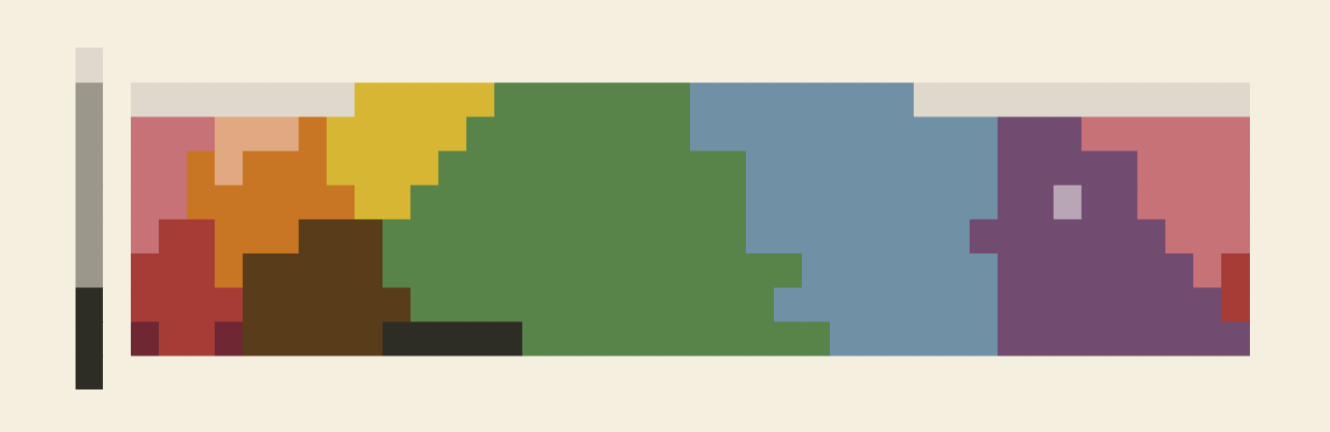
\includegraphics[width=0.49\textwidth]{docs/intro_rate_distortion/graphs/color_language.png}
            \caption{English on the colour palette from \citet{berlin1991basic}.
            }
            \label{fig:language_example}
        \end{figure}
    
    An example based on English is illustrated in Figure~\ref{fig:language_example}.
    To be specific, the colour chips in the green region will all be referred by the word ``green''.
    The boundary is hard in this example, but the naming policy $p(w|m)$ can have soft boundaries, e.g. by using Gaussian distribution.
    
    \item \textbf{interpretation policy $p(\hat{m}|w)$\label{par:decoder}}: an interpretation specifies the distribution of colour chips given a specific word, a.k.a. \emph{decoder} in standard information theory terminology, and can also be written as a function $I:\mathcal{W}\rightarrow\mathcal{C}$.
    Note we use $\hat{m}$ here instead of $m$ because the two random variables have different probability mass although they have the same sample space. 
    $\hat{m}$ is the understood or reconstructed meaning from the word $w$.
    For example, after receiving the word ``green'', we could have a distribution over all colours that is very similar to the one in Figure~\ref{fig:green_meaning} but more skewed towards blue.
    
    Following \citet{zaslavsky2018efficient}, an important assumption of this project is that mappings between $\hat{m}$ and $w$ are one-to-one, i.e.
    \begin{equation}
        p(\hat{m}|w) =
        \begin{cases}
            1 & \text{if $\hat{m}=w$}\\
            0 & \text{otherwise}
        \end{cases} 
        \label{eq:bijective_mhat_w}
    \end{equation}
    
    Rigorously speaking, $\hat{m}$ can't equal to $w$, but it is easier to write it this way. Therefore, the equivalence below holds:
    \begin{equation}
        p(c|w)  = \sum_{\hat{m}} p(c|\hat{m})p(\hat{m}|w)  = p(c|\hat{m})
        \label{eq:p_mhat_and_m}
    \end{equation}
    
    Similar to \citep{zaslavsky2018efficient}, by applying Bayes theorem, we can have the following equivalence:
    \begin{equation}
        \begin{split}
            & p(c|\hat{m}) = p(c|w) \\
            & = \sum_m p(c|m)p(m|w) \\
            & = \sum_m p(c|m) \frac{p(w|m)p(m)}{p(w)} \\
            & = \sum_m p(c|m) \frac{p(w|m)p(m)}{\sum_m p(w|m)p(m)}
        \end{split}
        \label{eq:bayesian_interpretation}
    \end{equation}
    That is, we can determine interpretation $p(c|w) = p(c|\hat{m})$ once we have an established language $p(w|m)$ and established meanings probability mass function $p(m)$.
\end{itemize}

\subsection{Full Derivation of Information Loss of a Language}
\label{appssec:derivation_of_info_loss}

The full derivation of Equation~\ref{eq:comm_info_loss} is given as follows:
\begin{equation}
   \begin{aligned}
        & \mathbb{E}_{p(\hat{m},m)}\left[D[m||\hat{m}]\right] \\
        & = \sum_{\hat{m},m,w} p(\hat{m}|w)p(w|m)p(m) \\ 
        & \cdot \sum_{c} p(c|m) \log \frac{p(c|m)}{p(c|w)} \\
        & = \sum_{\hat{m},m,w,c} p(\hat{m}|w)p(w|m)p(m)p(c|m)\log \frac{p(c|m)}{p(c|w)} \\
        & = \sum_{\hat{m},m,w,c} p(\hat{m}|w)p(w|m)p(m)p(c|m) \log p(c|m) \\
        & - \sum_{\hat{m},m,w,c} p(\hat{m}|w)p(w|m)p(m)p(c|m) \log p(c|w) \\ 
        & = \sum_{\hat{m},m,w,c} p(\hat{m}|w)p(w|m)p(m)p(c|m) \log \frac{p(c|m)}{p(c)} \\ 
        & - \sum_{\hat{m},m,w,c} p(\hat{m}|w)p(w|m)p(m)p(c|m) \log \frac{p(c|w)}{p(c)} \\ 
        & = \sum_{\hat{m},m,w,c} p(\hat{m},m,w,c) \log \frac{p(c|m)}{p(c)} \\
        & - \sum_{\hat{m},m,w,c} p(\hat{m},m,w,c) \log \frac{p(c|w)}{p(c)} \\ 
        & = \sum_{\cancel{\hat{m},w},m,c} p(\cancel{\hat{m},w},m,c) \log \frac{p(c|m)}{p(c)} \\ 
        & - \sum_{\cancel{\hat{m},m},w,c} p(\cancel{\hat{m},m},w,c) \log \frac{p(c|w)}{p(c)} \\ 
        & = \sum_{m,c} p(m,c) \log \frac{p(c|m)}{p(c)} \\ 
        & - \sum_{w,c} p(w,c) \log \frac{p(c|w)}{p(c)} \\ 
        & = {\sum_{m,c} p(m,c) \log \frac{p(c|m)p(m)}{p(c)p(m)}} \\ 
        & - {\sum_{w,c} p(w,c) \log \frac{p(c|w)p(w)}{p(c)p(w)}} \\  
        & = {I(M;C)} - {I(W;C)} 
    \end{aligned} 
     \label{eq:factorise_distortion}
\end{equation}


\subsection{Log-Likelihood as Information-Loss for the Learning Problem}
\label{appssec:ll_learning_loss}

In this section, we show why negative log-likelihood could be used as an alternative measure for the information loss of the learning problem. Suppose that the true distribution of colour chips and terms from the dataset $\mathcal{D}$ is $\mathcal{D}(w,c)$. Given then a data point ($w_n,c_n$) we have that $D(w,c)=1 \iff w=w_n \land c=c_n$ and we can calculate the KL-divergence between the true distribution and the learnt joint $p(w,c|H)$ as:
% Considering that $\mathcal{D}(c)$ is still a one-hot distribution, we can factorise the KL-divergence between $\mathcal{D}(c)$ and $p(c|H)$ as follows:
\begin{equation}
    \begin{split}
        & D[\mathcal{D}(w,c)||p(w,c|H)] \\ 
        & = \sum_{w,c} \mathcal{D}(w,c)\log \frac{\mathcal{D}(w,c)}{p(w,c|H)} \\
        & = \log \frac{1}{p(w=w_n,c=c_n|H)} \\
        & = -\log p(w_n,c_n|H)
    \end{split}
    \label{eq:learn_info_loss}
\end{equation}

Therefore, the negative log-likelihood is naturally a measure for the information loss in learning problem.

\end{document}
